% Build pipeline.pdf:
%   pdflatex -interaction=nonstopmode -jobname=pipeline pipeline_standalone.tex
\documentclass[tikz,border=6pt]{standalone}
\usepackage{tikz}
\usetikzlibrary{positioning,arrows.meta,calc}

\begin{document}
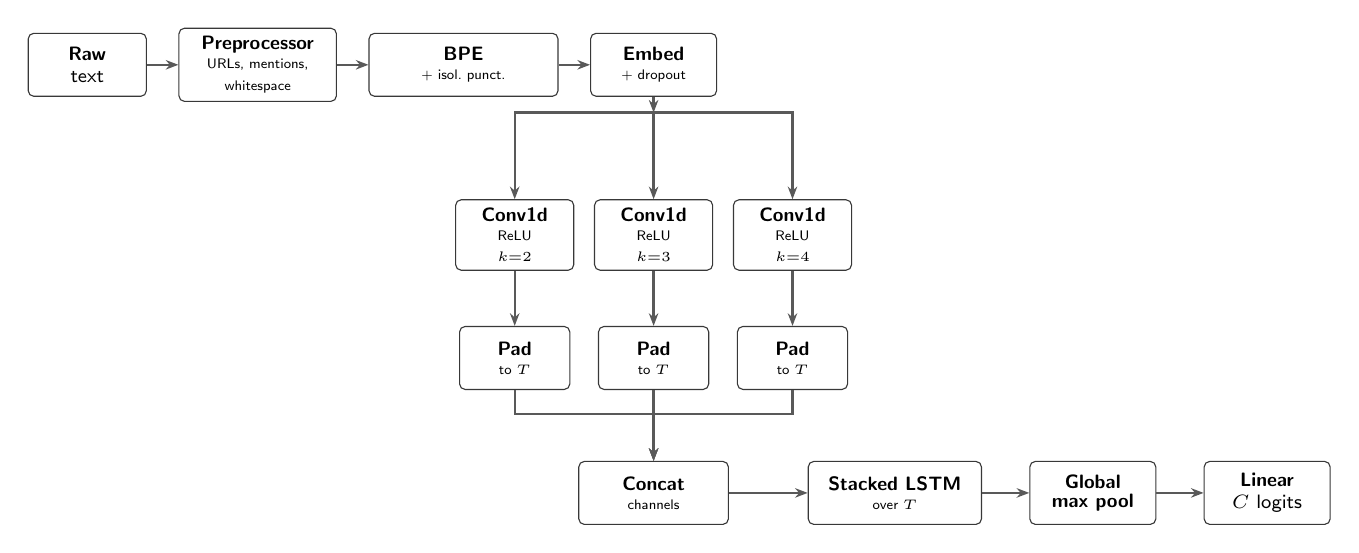
\begin{tikzpicture}[
  font=\sffamily\fontsize{6.8pt}{7.8pt}\selectfont,
  box/.style={
    rectangle,
    draw=black!78,
    rounded corners=2pt,
    inner sep=3pt,
    minimum height=8mm,
    align=center,
    fill=white,
  },
  kern/.style={-{Stealth[length=1.6mm]}, thick, draw=black!65},
]

  % --- Left: preprocessing chain ---
  \node[box, minimum width=15mm] (raw) {\textbf{Raw}\\text};
  \node[box, minimum width=20mm, right=4mm of raw] (pre) {\textbf{Preprocessor}\\[-1pt]\tiny URLs, mentions,\\\tiny whitespace};
  \node[box, minimum width=24mm, right=4mm of pre] (bpe) {\textbf{BPE}\\[-1pt]\tiny +\ isol.\ punct.};
  \node[box, minimum width=16mm, right=4mm of bpe] (emb) {\textbf{Embed}\\[-1pt]\tiny + dropout};

  \foreach \a/\b in {raw/pre, pre/bpe, bpe/emb} {
    \draw[kern] (\a.east) -- (\b.west);
  }

  % --- Embedding fans out to three CNN branches ---
  \node[box, minimum width=15mm, below left=13mm and 2mm of emb] (cv2) {\textbf{Conv1d}\\[-1pt]\tiny ReLU\\\tiny $k{=}2$};
  \node[box, minimum width=15mm, below=13mm of emb] (cv3) {\textbf{Conv1d}\\[-1pt]\tiny ReLU\\\tiny $k{=}3$};
  \node[box, minimum width=15mm, below right=13mm and 2mm of emb] (cv4) {\textbf{Conv1d}\\[-1pt]\tiny ReLU\\\tiny $k{=}4$};

  \coordinate (split) at ($(emb.south)+(0,-2mm)$);
  \draw[kern] (emb.south) -- (split);
  \draw[kern] (split) -| (cv2.north);
  \draw[kern] (split) -- (cv3.north);
  \draw[kern] (split) -| (cv4.north);

  \node[box, minimum width=14mm, below=7mm of cv2] (p2) {\textbf{Pad}\\[-1pt]\tiny to $T$};
  \node[box, minimum width=14mm, below=7mm of cv3] (p3) {\textbf{Pad}\\[-1pt]\tiny to $T$};
  \node[box, minimum width=14mm, below=7mm of cv4] (p4) {\textbf{Pad}\\[-1pt]\tiny to $T$};

  \draw[kern] (cv2) -- (p2);
  \draw[kern] (cv3) -- (p3);
  \draw[kern] (cv4) -- (p4);

  \node[box, minimum width=19mm, below=9mm of p3] (cat) {\textbf{Concat}\\[-1pt]\tiny channels};
  \draw[kern] (p2.south) -- ++(0,-3mm) -| (cat.north);
  \draw[kern] (p4.south) -- ++(0,-3mm) -| (cat.north);
  \draw[kern] (p3) -- (cat);

  \node[box, minimum width=22mm, right=10mm of cat] (ls) {\textbf{Stacked LSTM}\\[-1pt]\tiny over $T$};
  \node[box, minimum width=16mm, right=6mm of ls] (mx) {\textbf{Global}\\[-1pt]\textbf{max pool}};
  \node[box, minimum width=16mm, right=6mm of mx] (out) {\textbf{Linear}\\$C$ logits};

  \draw[kern] (cat.east) -- (ls.west);
  \draw[kern] (ls.east) -- (mx.west);
  \draw[kern] (mx.east) -- (out.west);

\end{tikzpicture}
\end{document}
